\documentclass[tikz,border=3pt]{standalone}
\usepackage{times}
\usepackage{xcolor}
\usepackage{tikz}
\usetikzlibrary{positioning}

\begin{document}
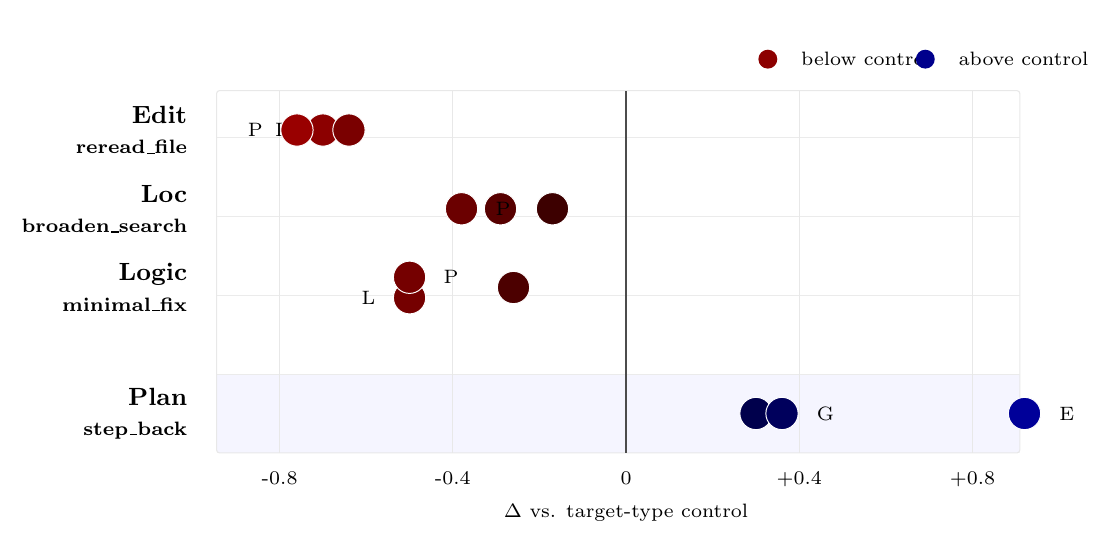
\begin{tikzpicture}[
  x=1mm,
  y=1mm,
  every node/.style={font=\rmfamily},
]
\path[use as bounding box] (-18,0) rectangle (114,62);

% Layout.
\def\xscale{55} % mm per delta unit
\def\xzero{58}

\newcommand{\dotpos}[4]{%
  \pgfmathsetmacro{\xx}{\xzero + (#1)*\xscale}
  \filldraw[fill=#3, draw=white, line width=0.35pt] (\xx,#2) circle (2.05);
}

% Step-back row highlight.
\fill[blue!4] (6,8) rectangle (108,18);

% Plot region.
\draw[gray!18, rounded corners=1pt] (6,8) rectangle (108,54);
\foreach \yy in {18,28,38,48} {
  \draw[gray!16] (6,\yy) -- (108,\yy);
}
\foreach \d/\lab in {-0.8/-0.8,-0.4/-0.4,0/0,+0.4/+0.4,+0.8/+0.8} {
  \pgfmathsetmacro{\xx}{\xzero + (\d)*\xscale}
  \draw[gray!18] (\xx,8) -- (\xx,54);
  \node[font=\scriptsize, anchor=north] at (\xx,6.8) {\lab};
}
\draw[black!70, line width=0.55pt] (\xzero,8) -- (\xzero,54);
\node[font=\scriptsize, anchor=north] at (58,2.8) {$\Delta$ vs. target-type control};

% Minimal legend.
\fill[red!55!black] (76,58) circle (1.2);
\node[font=\scriptsize, anchor=west] at (79,58) {below control};
\fill[blue!55!black] (96,58) circle (1.2);
\node[font=\scriptsize, anchor=west] at (99,58) {above control};

% Row labels.
\node[font=\bfseries\small, anchor=east, align=right] at (3.5,49) {\textsc{Edit}\\{\scriptsize reread\_file}};
\node[font=\bfseries\small, anchor=east, align=right] at (3.5,39) {\textsc{Loc}\\{\scriptsize broaden\_search}};
\node[font=\bfseries\small, anchor=east, align=right] at (3.5,29) {\textsc{Logic}\\{\scriptsize minimal\_fix}};
\node[font=\bfseries\small, anchor=east, align=right] at (3.5,13) {\textsc{Plan}\\{\scriptsize step\_back}};

% Explicit x positions for labeled points.
\pgfmathsetmacro{\xEditL}{\xzero + (-0.70)*\xscale}
\pgfmathsetmacro{\xEditP}{\xzero + (-0.76)*\xscale}
\pgfmathsetmacro{\xLocP}{\xzero + (-0.38)*\xscale}
\pgfmathsetmacro{\xLogicL}{\xzero + (-0.50)*\xscale}
\pgfmathsetmacro{\xLogicP}{\xzero + (-0.50)*\xscale}
\pgfmathsetmacro{\xPlanE}{\xzero + (0.92)*\xscale}
\pgfmathsetmacro{\xPlanG}{\xzero + (0.36)*\xscale}

% Off-diagonal transfers only.
% Edit strategy.
\dotpos{-0.70}{49}{red!55!black}{Loc}
\node[font=\scriptsize, anchor=east] at (\xEditL - 3.1,49) {L};
\dotpos{-0.64}{49}{red!48!black}{Logic}
\dotpos{-0.76}{49}{red!60!black}{Plan}
\node[font=\scriptsize, anchor=east] at (\xEditP - 3.1,49) {P};

% Loc strategy.
\dotpos{-0.29}{39}{red!34!black}{Edit}
\dotpos{-0.17}{39}{red!24!black}{Logic}
\dotpos{-0.38}{39}{red!42!black}{Plan}
\node[font=\scriptsize, anchor=west] at (\xLocP + 3.1,39) {P};

% Logic strategy.
\dotpos{-0.26}{29}{red!30!black}{Edit}
\dotpos{-0.50}{27.7}{red!46!black}{Loc}
\node[font=\scriptsize, anchor=east] at (\xLogicL - 3.1,27.7) {L};
\dotpos{-0.50}{30.3}{red!46!black}{Plan}
\node[font=\scriptsize, anchor=west] at (\xLogicP + 3.1,30.3) {P};

% Plan strategy.
\dotpos{+0.92}{13}{blue!60!black}{Edit}
\node[font=\scriptsize, anchor=west] at (\xPlanE + 3.2,13) {E};
\dotpos{+0.30}{13}{blue!30!black}{Loc}
\dotpos{+0.36}{13}{blue!36!black}{Logic}
\node[font=\scriptsize, anchor=west] at (\xPlanG + 3.2,13) {G};

\end{tikzpicture}
\end{document}
